\documentclass{report}
\usepackage{graphicx}

\usepackage{amsmath}
\DeclareMathOperator*{\argmax}{argmax}

\usepackage{hyperref}
\hypersetup{
    colorlinks=true,
    linkcolor=blue,
    filecolor=magenta,      
    urlcolor=cyan,
}

\begin{document}

\title{Banana World Project Report}
\author{Denis Sergeev}


\section*{Problem definition}

The goal of the project was to create a RL Agent which is able to train from scratch by interacting with the Banana World environment for a series of episodes. During the episode the agent receives the environment state. The agent is able to perform some actions which may change the environment state.

\subsection*{Environment description}
The \textbf{state space} has \(37\) dimensions each of which is a continuous variable. It includes the agent's velocity, along with ray-based perception of objects around the agent's forward direction. The \textbf{action space} contains the following \(4\) legal actions:
\begin{itemize}
  \item move forward \(0\)
  \item move backward \(1\)
  \item turn left \(2\)
  \item turn right \(3\)
\end{itemize}
A reward of \(+1\) is provided for collecting a yellow banana, and a reward of \(-1\)` is provided for collecting a blue banana. Thus, the goal of the agent is to collect as many yellow bananas as possible while avoiding blue bananas. The task is episodic, and in order to solve the environment, the agent must get an average score of \(+13\) over \(100\) consecutive episodes.


\section*{Solution}
\subsection*{Deep Q-Network Architecture}
\subsubsection*{Network}
Since the agent should act upon environment state provided as vector of size \(37\), I decided to build simple network with \(3\) fully connected layers, which should predict the Q-value for each action given the input state. The input has size 37, output 4. I tried 64x64, 64x32, 32x32, 32x16 hidden layers configuration. The best one was 32x32, since it was able to reach the training goal faster and it has less internal parameters then 64x64 and 64x32.

\subsection*{Training}
\subsubsection*{Loss function and optimizing method}

I tried 2 loss functions \ref{loss}: Simple DQN loss \ref{dqn-loss} and \href{https://arxiv.org/pdf/1509.06461.pdf}{Double DQN loss} \ref{ddqn-loss}
\begin{equation} \label{loss}
L \equiv (Y_{t} - Q(S_{t}, a; \theta_{t}))^{2}
\end{equation}
\begin{equation} \label{dqn-loss}
Y_t \equiv R_{t+1} + \gamma \max_a Q(S_t, a; \theta'_t)
\end{equation}
\begin{equation} \label{ddqn-loss}
Y_t \equiv R_{t+1} + \gamma Q(S_{t+1}, \argmax_a Q(S_t, a; \theta_t); \theta'_t)
\end{equation}
Where \(Q(S_t, a, \theta_t)\) is output (value of action \(a\)) of the network with internal parameters \(\theta_t\) given input \(S_t\). Both loss functions used 2 sets of network parameters: target \(\theta'_t\) and local \(\theta_t\). Target network parameters was updating through soft update \(\theta'_t = (1 - \tau) \theta'_t + \tau \theta_t\).
As optimizing method for \(\theta_t\) I used Adam with learning rate \(\alpha\).

\subsubsection*{Experience replay}

The input for training did not come directly from episodes. Instead I used experience replay technique (see \href{https://storage.googleapis.com/deepmind-media/dqn/DQNNaturePaper.pdf}{Human-level control through deep reinforcement learning}).


\section*{Results}

I came up using following training hyper parameters:
\begin{itemize}
	\item \(\epsilon_{start}\): 1.0, \(\epsilon_{end}\): 0.01, \(\epsilon_{decay}\): 0.97
	\item Buffer size: 100000
	\item Batch size: 64
	\item \(\gamma\): 0.99
	\item \(\tau\): 0.005
	\item \(\alpha\): 0.0005
\end{itemize}
They were used across all training experiments below.


\subsection*{Training DDQN 32x16}

DQN architecture: fully connected with bias 37x32x16x4. Loss \ref{ddqn-loss}.

Training history:

Episode 100.	Average Score: 4.88.	Time elapsed: 4:35

Episode 200.	Average Score: 12.21.	Time elapsed: 9:11

Environment solved in 170 episodes!	Average Score: 13.12. Time elapsed: 12:31s. See \ref{fig:DDQN_32x16}.

\begin{figure}
	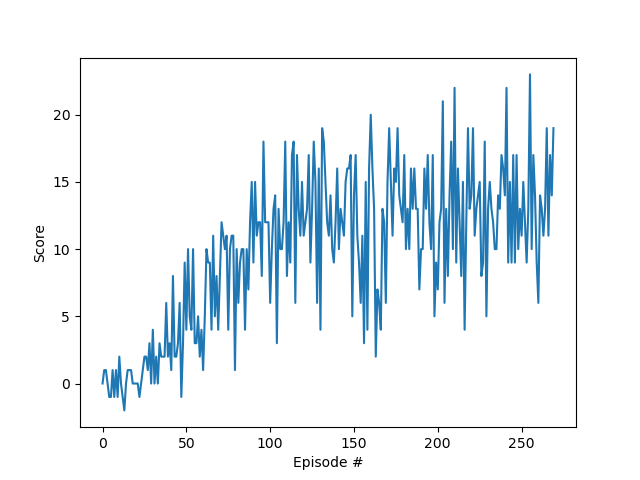
\includegraphics[width=0.9\linewidth]{res/DDQN_32x16/score.png}
	\caption{DDQN 32x16: Rewards per episode}
	\label{fig:DDQN_32x16}
\end{figure}


\subsection*{Training DDQN 32x32}

DQN architecture: fully connected with bias 37x32x32x4. Loss \ref{ddqn-loss}.

Training history:

Episode 100.	Average Score: 6.50.	Time elapsed: 3:26

Episode 200.	Average Score: 12.66.	Time elapsed: 6:51

Environment solved in 109 episodes!	Average Score: 13.08. Time elapsed: 7:09s. See \ref{fig:DDQN_32x32}.

\begin{figure}
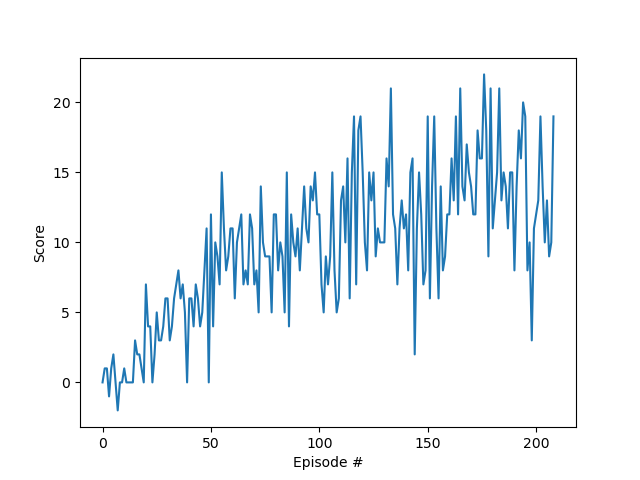
\includegraphics[width=0.9\linewidth]{res/DDQN_32x32/score.png}
\caption{DDQN 32x32: Rewards per episode}
\label{fig:DDQN_32x32}
\end{figure}


\subsection*{Training DDQN 64x32}

DQN architecture: fully connected with bias 37x64x32x4. Loss \ref{ddqn-loss}.

Training history:

Episode 100.	Average Score: 5.69.	Time elapsed: 3:25

Episode 200.	Average Score: 12.38.	Time elapsed: 6:52

Environment solved in 118 episodes!	Average Score: 13.06. Time elapsed: 7:33s. See \ref{fig:DDQN_64x32}.

\begin{figure}
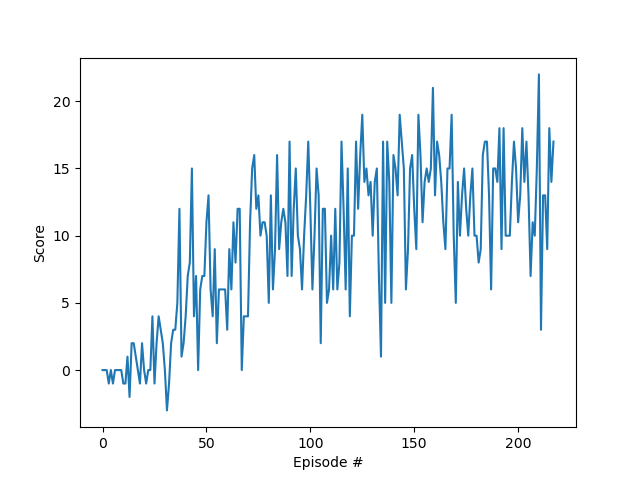
\includegraphics[width=0.9\linewidth]{res/DDQN_64x32/score.png}
\caption{DDQN 64x32: Rewards per episode}
\label{fig:DDQN_64x32}
\end{figure}


\subsection*{Training DQN 64x32}

DQN architecture: fully connected with bias 37x64x32x4. Loss \ref{dqn-loss}.

Training history:

Episode 100.	Average Score: 4.75.	Time elapsed: 3:10

Episode 200.	Average Score: 11.97.	Time elapsed: 6:22

Environment solved in 136 episodes!	Average Score: 13.02. Time elapsed: 7:31s. See \ref{fig:DQN_64x32}.

\begin{figure}
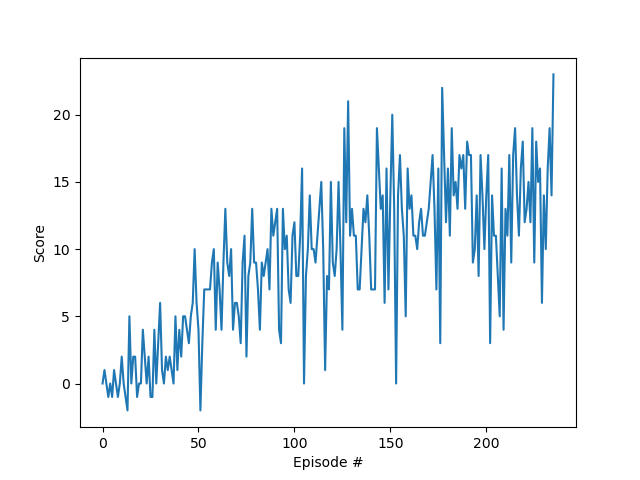
\includegraphics[width=0.9\linewidth]{res/DQN_64x32/score.png}
\caption{DQN 64x32: Rewards per episode}
\label{fig:DQN_64x32}
\end{figure}


\subsection*{Training DQN 64x64}

DQN architecture: fully connected with bias 37x64x64x4. Loss \ref{dqn-loss}.

Training history:

Episode 100.	Average Score: 4.75.	Time elapsed: 3:21

Episode 200.	Average Score: 10.90.	Time elapsed: 6:39

Environment solved in 130 episodes!	Average Score: 13.03. Time elapsed: 7:38s. See \ref{fig:DQN_64x64}.

\begin{figure}
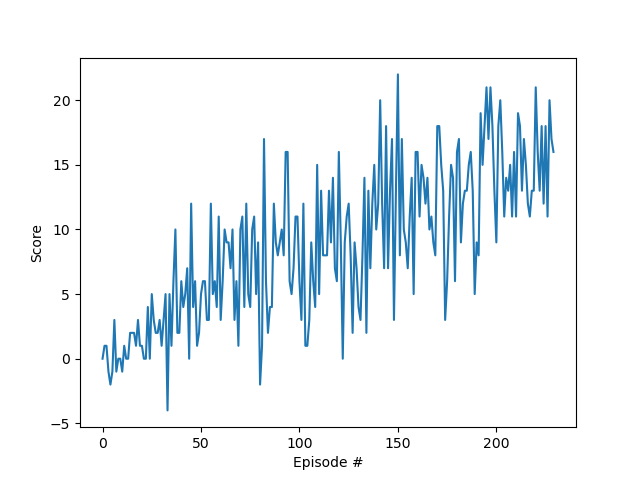
\includegraphics[width=0.9\linewidth]{res/DQN_64x64/score.png}
\caption{DQN 64x64: Rewards per episode}
\label{fig:DQN_64x64}
\end{figure}

\subsection*{Conclusion}

From the above results we can summarize, that DDQN has slightly better training performance. Also 32x32 hidden layer configuration is the best. It was trained faster and has few internal parameters.


\section*{Areas of improvement}

During evaluation of the trained agent I noticed, that in some cases the agent hangs up. It begins alternating between 2 positions. You may see it at the end of the video I uploaded on \href{https://youtu.be/PPSJ2k9RBq0}{youtube}. This is caused by the fact, that the agent makes its decision based only on instant state. It does not take into account previous states and actions. Intuitively is clear that the agent needs some memory to store previous actions and states. This could be achieved by \href{http://cs229.stanford.edu/proj2016/report/ChenYingLaird-DeepQLearningWithRecurrentNeuralNetwords-report.pdf}{adding recurrent unit to the network}, like LSTM, GRU or just simple RNN.
Another improvement could be implementing \href{https://arxiv.org/abs/1511.05952}{prioritized experience replay}.

\end{document}
